\section{Description séquentielle des modules}
    \label{sec:modules}
    
Les diagrammes de séquences présentés dans cette partie ont pour objectif d'illustrer le fonctionnement des trois principales fonctionnalités de Glasir, à savoir le filtrage, l'optimisation et l'édition de paramètres de synthèse.

Chaque diagramme commence par l'ouverture d'un arbre avec Glasir, représenté par le bloc "Start".

	\subsection{Filtre}

	    \begin{figure}[H]
	        \centering
	        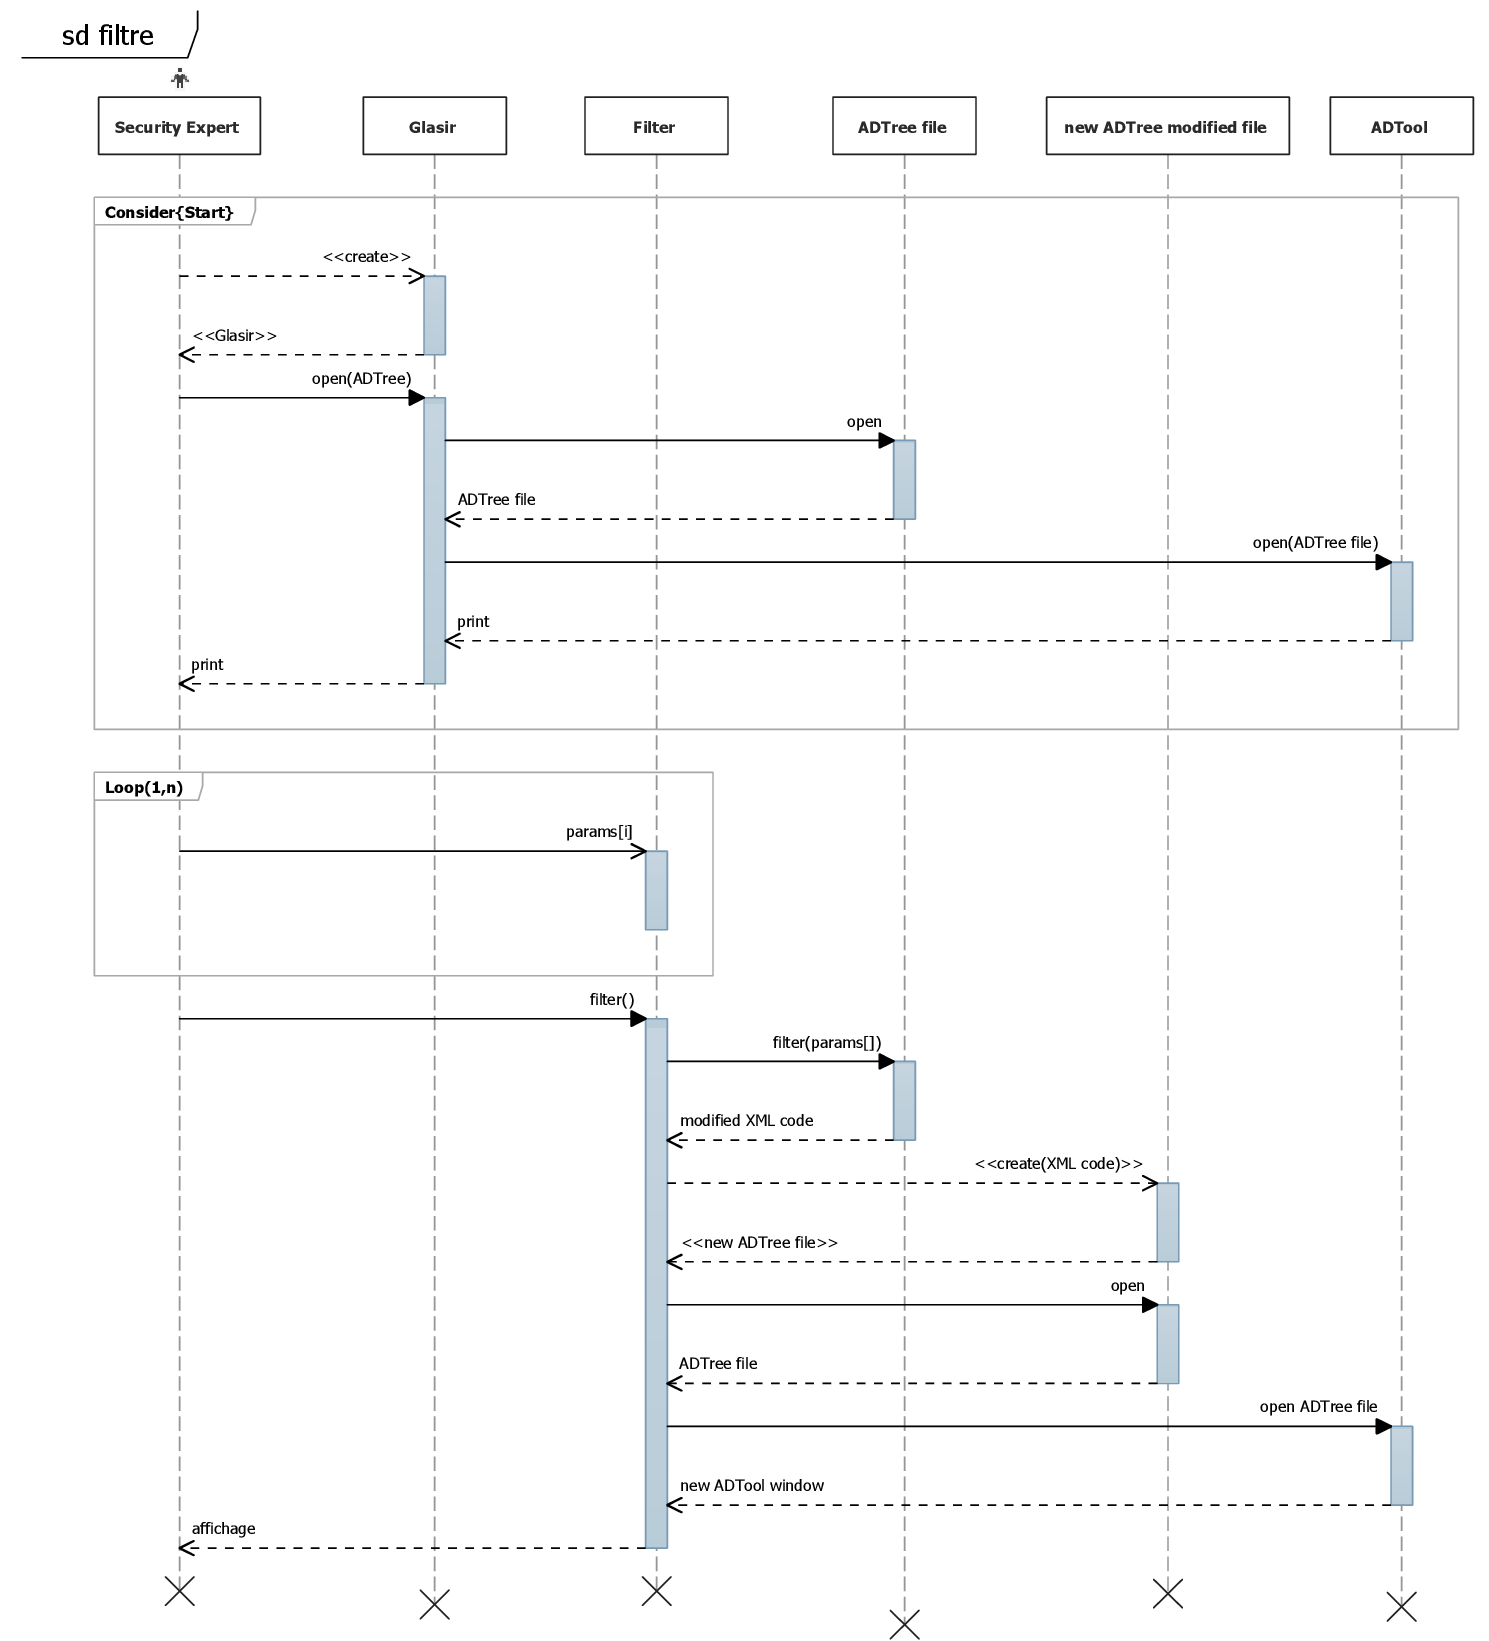
\includegraphics[height=1\textwidth]{figure/Filter.png}
	        \caption{Diagramme de séquence du module Filtre.}
	        \label{fig:filter}
	    \end{figure}

Pour réaliser le filtrage d'un arbre, l'expert en sécurité va passer en paramètre au filtre les différents intervalles de filtrage des valuations de l'arbre. Il va ensuite lancer le filtre. Celui-ci va analyser le code XML de l'arbre afin d'obtenir le code XML de l'arbre filtré. Il va alors créer un nouveau fichier XML dans lequel va être inscrit ce code. Et enfin l'arbre filtré va être affiché dans un nouvel onglet d'ADTool.

	\subsection{Optimiseur}

	    \begin{figure}[H]
	        \centering
	        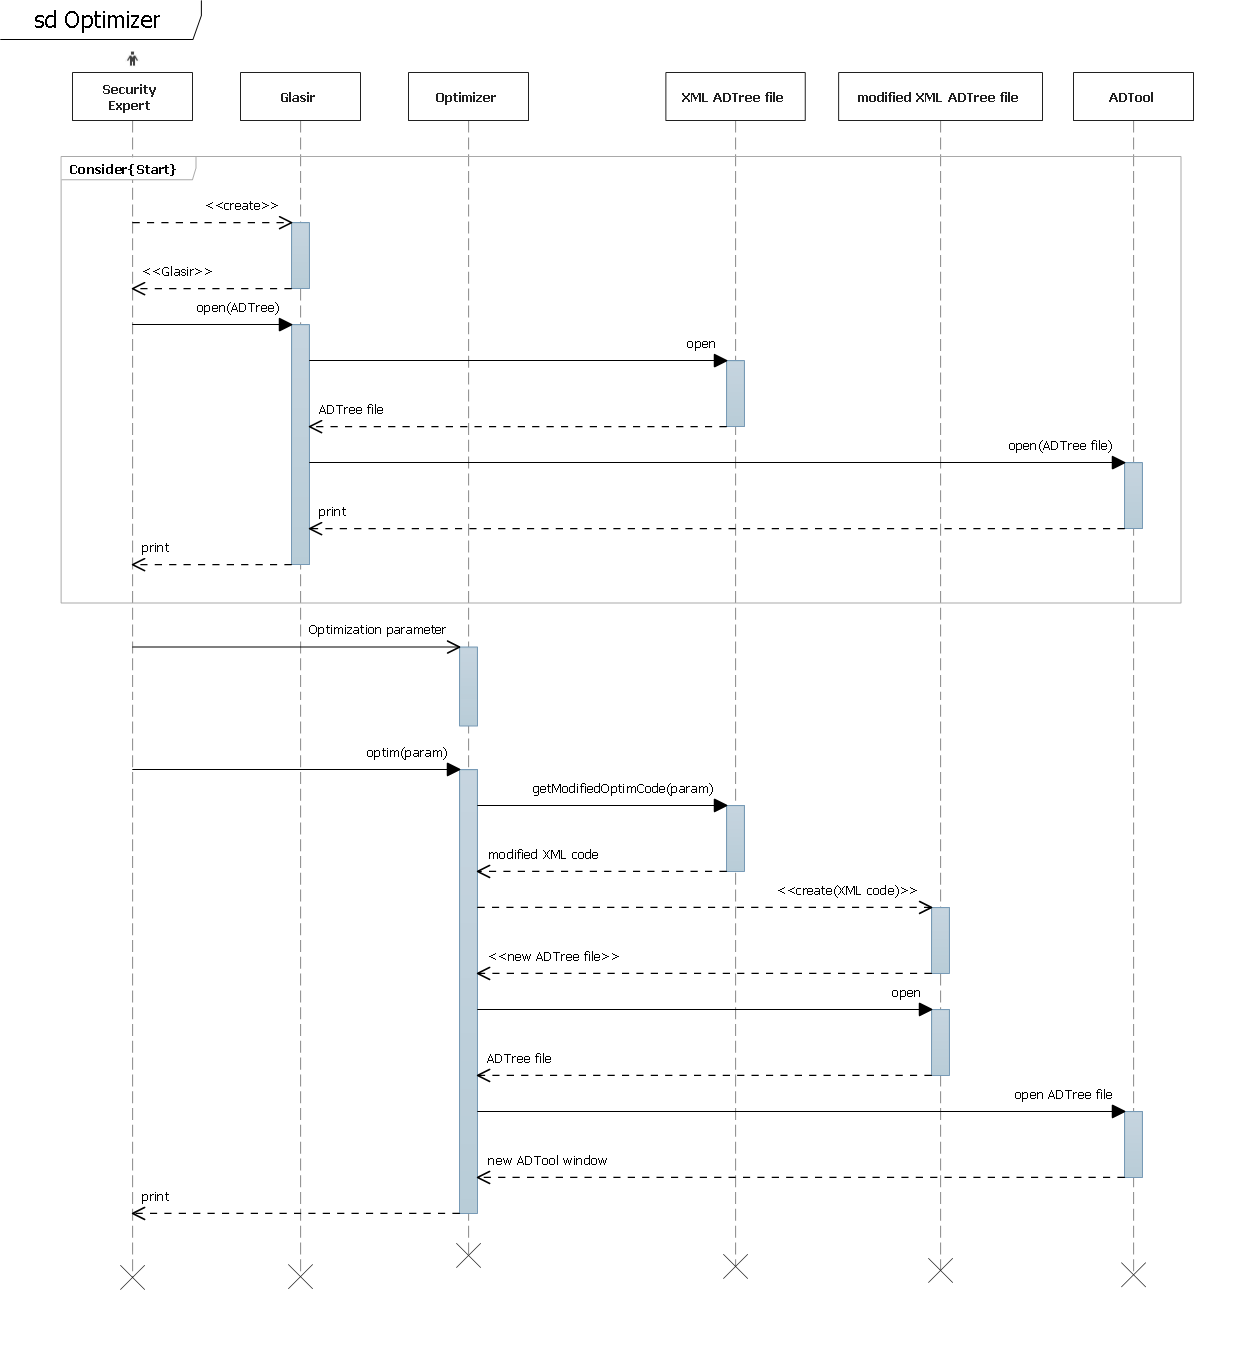
\includegraphics[height=1\textwidth]{figure/Optim.png}
	        \caption{Diagramme de séquence du module Optimiseur.}
	        \label{fig:optim}
	    \end{figure}

Pour réaliser l'optimisation d'un arbre, l'expert en sécurité va passer en paramètre la valuation de l'arbre selon laquelle il veut l'optimiser. Il va ensuite lancer l'optimiseur. Celui-ci va analyser le code XML de l'arbre afin d'obtenir le code XML de l'arbre optimisé. Il va alors créer un nouveau fichier XML dans lequel va être inscrit ce code. Et enfin l'arbre optimisé va être affiché dans un nouvel onglet d'ADTool.

	\subsection{Éditeur de fonctions}

	    \begin{figure}[H]
	        \centering
	        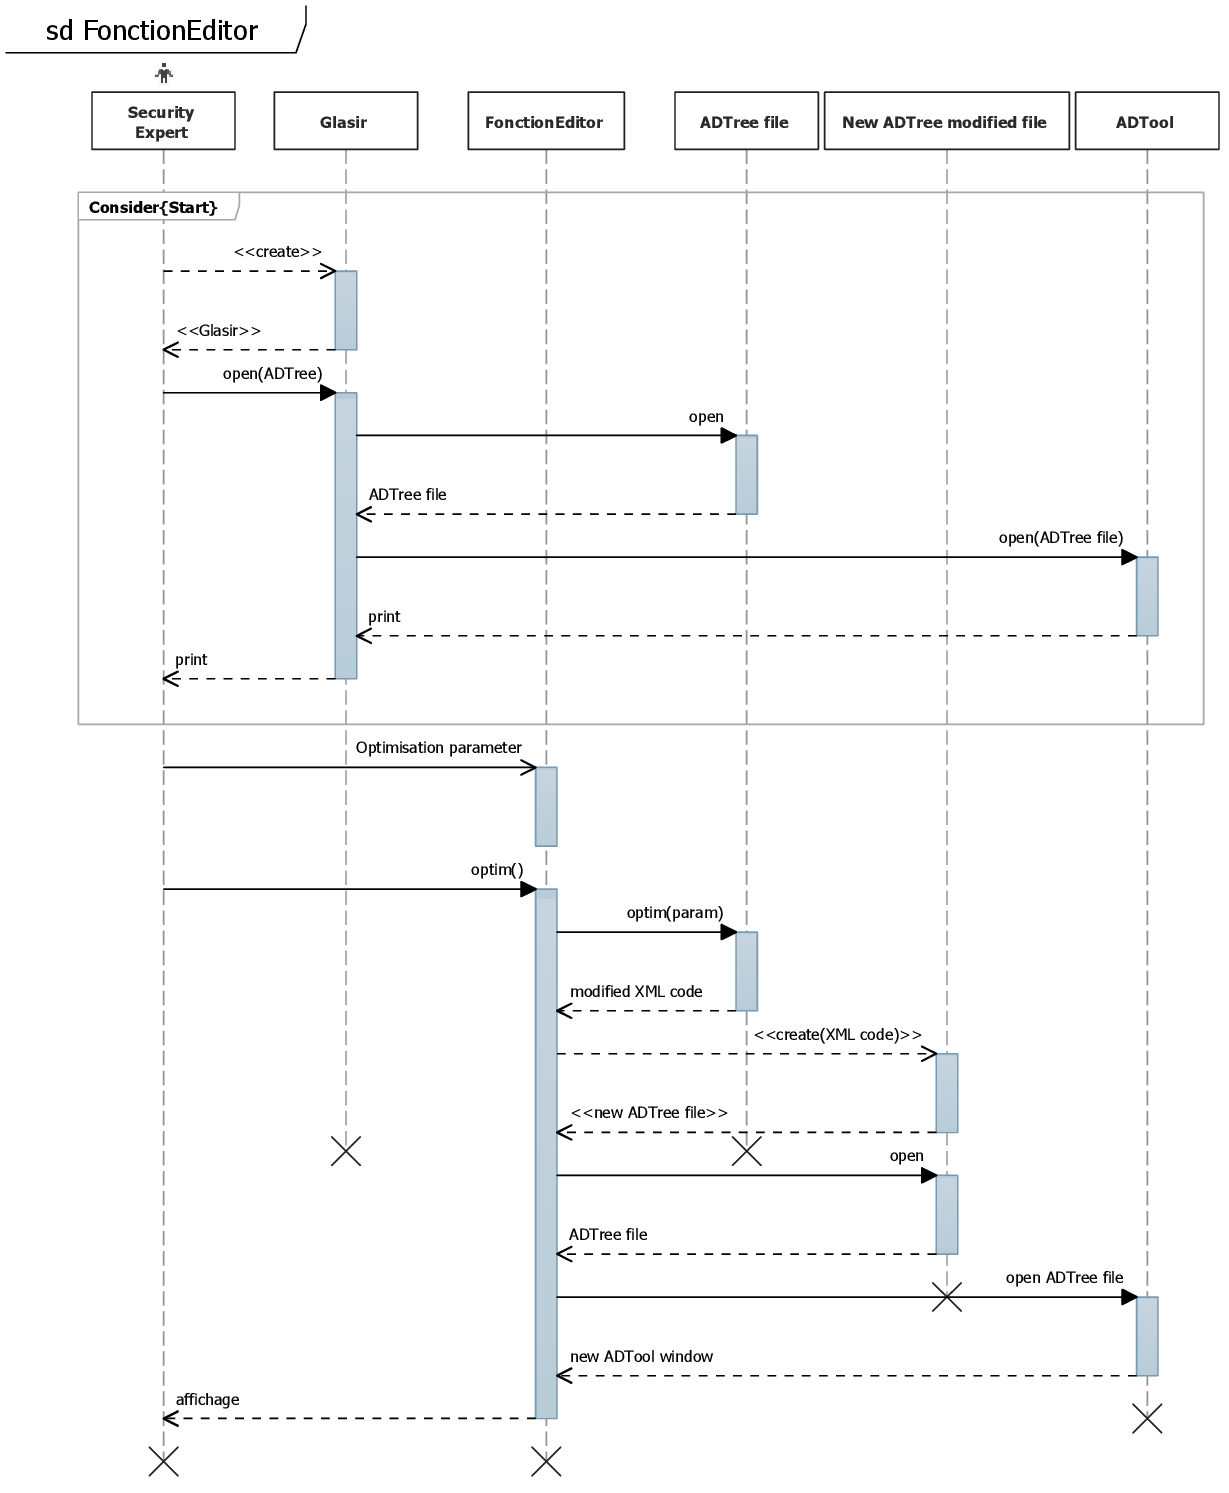
\includegraphics[height=1\textwidth]{figure/FunctionEditor.png}
	        \caption{Diagramme de séquence du module Éditeur de fonctions.}
	        \label{fig:function}
	    \end{figure}

Pour ajouter un paramètre de synthèse à l'arbre, l'expert en sécurité va commencer par écrire la fonction de calcul de ce paramètre en fonction des valuations déjà présentes. Il va ensuite lancer l'éditeur de fonctions. Celui-ci va analyser le code XML de l'arbre afin de génerer le code XML de l'arbre avec la valuation supplémentaire. Il va alors créer un nouveau fichier XML dans lequel va être inscrit ce code. Et enfin le nouvel arbre va être affiché dans un nouvel onglet d'ADTool.